\documentclass[a4paper,12pt]{article}
%\usepackage[ngerman]{babel}
\usepackage[utf8]{inputenc}
%
\usepackage[paper=a4paper,dvips,top=10mm,left=30mm,right=30mm,foot=10mm,bottom=20mm]{geometry}
%
%\usepackage{times}

\usepackage{graphicx}
%\DeclareGraphicsExtensions{.pdf,.png,.jpg}
\usepackage{pstricks}
%\usepackage{auto-pst-pdf}
%\usepackage{graphics}
%\usepackage[fleqn]{amsmath}
\usepackage{amsmath}
%\usepackage{mathptmx}
%\usepackage{amsfonts}
\usepackage{amssymb}
\usepackage{amsthm}
\usepackage{amsopn}
\usepackage{xspace}
\usepackage{array}
\usepackage{epsfig}
\usepackage{caption}
\usepackage{subcaption}
\usepackage{booktabs}
\usepackage{wrapfig}

\usepackage{multicol}

%\usepackage{multirow}
\usepackage{subfig}
%
\usepackage{algpseudocode}
%\usepackage[chapter]{algorithm}
%
%
\usepackage{color} %needed by gnuplot
\definecolor{comment}{rgb}{.5,.5,.5}
%
%
%
%
\usepackage{titlesec}
%
%% making chapter titles pretty
%\titlespacing*{\chapter}{0pt}{-50pt}{20pt}
%\titleformat{\chapter}[display]{\normalfont\huge\bfseries}{\chaptertitlename\ \thechapter}{20pt}{\Huge}
%\titleformat{\chapter}{\normalfont\LARGE\bfseries}{\chaptertitlename \thechapter}{20pt}{\LARGE}
%\renewcommand{\chaptername}{}
%
%
\numberwithin{figure}{section}
%
%\newcommand\CC{\Lang{\mbox{R}}\xspace}
%\newcommand\Lang[1]{\textsc{#1}}
%\newcommand{\kw}[1]{\texttt{\textbf{#1}}}
%\newcommand{\cd}[1]{\texttt{#1}}
\newcommand{\HRule}{\rule{\linewidth}{0.2mm}\\}
%
\newcommand\Exp{\ensuremath{\mathbb{E}}\xspace}
\newcommand\Var{\ensuremath{\mathbb{V}}\xspace}

\renewcommand\Pr{\ensuremath{\text{Pr}}\xspace}

\newcommand\F{\ensuremath{\mathbb{F}}\xspace}

\newcommand\N{\ensuremath{\mathbb{N}}\xspace}
\newcommand\Z{\ensuremath{\mathbb{Z}}\xspace}
\newcommand\Q{\ensuremath{\mathbb{Q}}\xspace}
\newcommand\R{\ensuremath{\mathbb{R}}\xspace}
\newcommand\C{\ensuremath{\mathbb{C}}\xspace}
\newcommand\I{\ensuremath{\mathbb{I}}\xspace}
%
\newcommand\norm[1]{\ensuremath{\lVert#1\rVert}}
\newcommand\abs[1]{\ensuremath{\lvert#1\rvert}}
\newcommand\ceil[1]{\ensuremath{\lceil#1\rceil}}
\newcommand\floor[1]{\ensuremath{\lfloor#1\rfloor}}
\newcommand\set[1]{\ensuremath{\{#1\}}}
\newcommand\angular[1]{\ensuremath{\langle#1\rangle}}
%
\newcommand\Norm[1]{\ensuremath{\left\lVert#1\right\rVert}}
\newcommand\Abs[1]{\ensuremath{\left\lvert#1\right\rvert}}
\newcommand\Ceil[1]{\ensuremath{\left\lceil#1\right\rceil}}
\newcommand\Floor[1]{\ensuremath{\left\lfloor#1\right\rfloor}}
\newcommand\Set[1]{\ensuremath{\left\{#1\right\}}}
\newcommand\Angular[1]{\ensuremath{\left\langle#1\right\rangle}}
%
\newcommand\Tr{\ensuremath{\text{Tr}}}
%\newcommand\dom{\ensuremath{\mathbf{dom}}}
\newcommand\dom[1]{\unskip\ensuremath{\,\mathbf{dom}(#1)}}
%
%\DeclareMathOperator{\dom}{\mathbf{dom}}
%
\newcommand\laplacian{\ensuremath{\mathcal{L}}}
\newcommand\SO[1]{\ensuremath{\mathbf{SO}(#1)}}
\newcommand\var[1]{\ensuremath{\mathbf{var}(#1)}}
\newcommand\EIG[1]{\ensuremath{\mathbf{EIG}(#1)}}
\newcommand\0{\ensuremath{\mathbf{0}}}
\newcommand\1{\ensuremath{\mathbf{1}}}
\newcommand\B{\ensuremath{\mathbf{B}}}
\newcommand\U{\ensuremath{\mathbf{U}}}
\newcommand\nextt{\ensuremath{\mathrm{next}}}
%
%
%% Define a label for every chapter and section, which has the same name as the entity
%\newcommand{\Chapter}[1]{\chapter{#1} \label{ch:#1}}
\newcommand{\Section}[1]{\section{#1} \label{sec:#1}}
\newcommand{\Subsection}[1]{\subsection{#1} \label{ssec:#1}}
%
%
%\newcommand{\LOOM}{\ensuremath{\cal{LOOM}}\xspace}
%\newcommand{\PolyTOIL}{\textbf{PolyTOIL}\xspace}
%
\newtheorem{theorem}{Theorem}[section]
\newtheorem{definition}[theorem]{Definition}
\newtheorem{lemma}[theorem]{Lemma}
\newtheorem{corollary}[theorem]{Corollary}
\newtheorem{fact}[theorem]{Fact}
\newtheorem{observation}[theorem]{Observation}
\newtheorem{example}[theorem]{Example}
%% theorems without counter
\newtheorem*{notation}{Notation}
\newtheorem*{notation*}{Notation}
%
\renewcommand{\algorithmicrequire}{\textbf{Input:}}
\renewcommand{\algorithmicensure}{\textbf{Output:}}

%
%\newcommand\Cls[1]{\textsf{#1}}
%\newcommand\Fig[1]{Figure~\ref{Figure:#1}}
%
%\usepackage{labels}
\usepackage{equation}
%\usepackage{prog2tex}
%
%
\usepackage{prettyref}
\usepackage{titleref}
%\usepackage{hyperref}
%
%%% Algorithm %%%
\newrefformat{alg}{Algorithm~(\ref{#1})}%\glqq\titleref{#1}\grqq \ auf Seite \pageref{#1}}
%%% Equations %%%
\newrefformat{eq}{Equation~(\ref{#1})}%\glqq\titleref{#1}\grqq \ auf Seite \pageref{#1}}
%%% Problem %%%
\newrefformat{pr}{Problem~(\ref{#1})}%\glqq\titleref{#1}\grqq \ auf Seite \pageref{#1}}
%%% Definition %%%
\newrefformat{def}{Definition~\ref{#1}}%\glqq\titleref{#1}\grqq \ auf Seite \pageref{#1}}
%%% Figures %%%
\newrefformat{fig}{Figure~(\ref{#1})} %\glqq\titleref{#1}\grqq \ auf Seite \pageref{#1}}
%%% Tables %%%
\newrefformat{tab}{Table~(\ref{#1})} %\glqq\titleref{#1}\grqq \ auf Seite \pageref{#1}}
%
\newrefformat{th}{Theorem~(\ref{#1})} %\glqq\titleref{#1}\grqq \ auf Seite \pageref{#1}}
%
\newrefformat{ch}{Chapter~\ref{#1}} %\glqq\titleref{#1}\grqq \ auf Seite \pageref{#1}}
%
\newrefformat{sec}{Section~\ref{#1}} %\glqq\titleref{#1}\grqq \ auf Seite \pageref{#1}}
%
\newrefformat{ssec}{Subsection~\ref{#1}} %\glqq\titleref{#1}\grqq \ auf Seite \pageref{#1}}
%
\newcommand\parenref[1]{(\ref{#1})}

%\def\listofnotations{\input{notation} \clearpage}
%\def\addnotation #1: #2#3{$#1$\> \parbox{5in}{#2 \fill  \pageref{#3}}\\}
%\def\newnot#1{\label{#1}}

%\usepackage[refpage]{nomencl}
\usepackage{nomencl}
\makenomenclature
%\renewcommand{\nomname}{List of Notations}
%\renewcommand*{\pagedeclaration}[1]{\unskip\dotfill\hyperpage{#1}}
%\nomlabelwidth=25mm
 
%\usepackage{makeidx}
%\makeindex

\usepackage{comment}
%\includecomment{comment}
%
%\newenvironment{excerpt}{\begin{quote}\begin{minipage}\textwidth}{\end{minipage}\end{quote}}
%
%\renewcommand{\textfraction}{0.01}
%
\begin{document}
\vspace{-50pt}
\title{
\includegraphics[width=0.20\textwidth]{uni-jena-logo.pdf}\\
				A brief survey of Plagiarism detection software
        }
\author{%Fakultät für Mathematik und Informatik\\
        Faculty of Mathematics and Computer Science\\
        %Friedrich Schiller Universität Jena\\
        Friedrich Schiller University Jena\\ 
        \rule{\textwidth}{0.5pt}\\
        {Daniel Baak}\\
        \texttt{daniel.baak@uni-jena.de}\\[-8pt]
        \rule{\textwidth}{0.5pt}\\
        Advisor: Prof. Dr. Eberhard Zehendner
        \vspace{\fill}
        }
\date{Lyon, \today}

\maketitle

%
\begin{abstract}
It has become exceedingly simple to communicate and share information thanks to inventions such like personal computers and the Internet. Moreover it has become trivial to just copy the raw information and leave out annoyances such as references as to where the information originated from or who is the author, a practice which in one word can be summarized as plagiarism. This practice is dreaded in academia and the industry for obvious reasons making the idea of automatically detecting it very attractive. 

This article presents a hierarchy of the types of plagiarism that can arise in documents, as well as known algorithmic methods for detecting them. The main focus lies on detecting signs indicating possible plagiarism in scientific articles. On a sideline we will cover some methods for detecting plagiarism in the source code of computer programs. Finally we'll look into a few of the available software packages that promise to simplify the process of review in academia.
\end{abstract}

%
\section{Introduction}
In order not to run off onto a holy war against anything that some software package highlights in red, we shall begin with a word of caution. Computer programs can only show the values of certain similarity measures between documents as well as text fragments that are similar or identical, but none of these things as of itself is a clear verdict for a case of plagiarism. Many times on-line solutions parse a document, just to find out that the exact same text is already in the library. This can mean either of two things: 
\begin{enumerate}
\item the new document is a plagiarized copy
\item the document has already been submitted to the library
\end{enumerate}

In some fields it may be a well footed practice to copy large fragments from previous works in order to support ones point, one example may be legal texts.

Not only is a document which the plagiarism detection software (from now on referred to as PDS) labels as being plagiarized not necessarily such, also a document which the PDS labels to be original work not always such. PDS should be viewed as a tool, and as any tool it may work great in the right hands or just not do it's job well at all in the wrong hands.


\begin{figure}
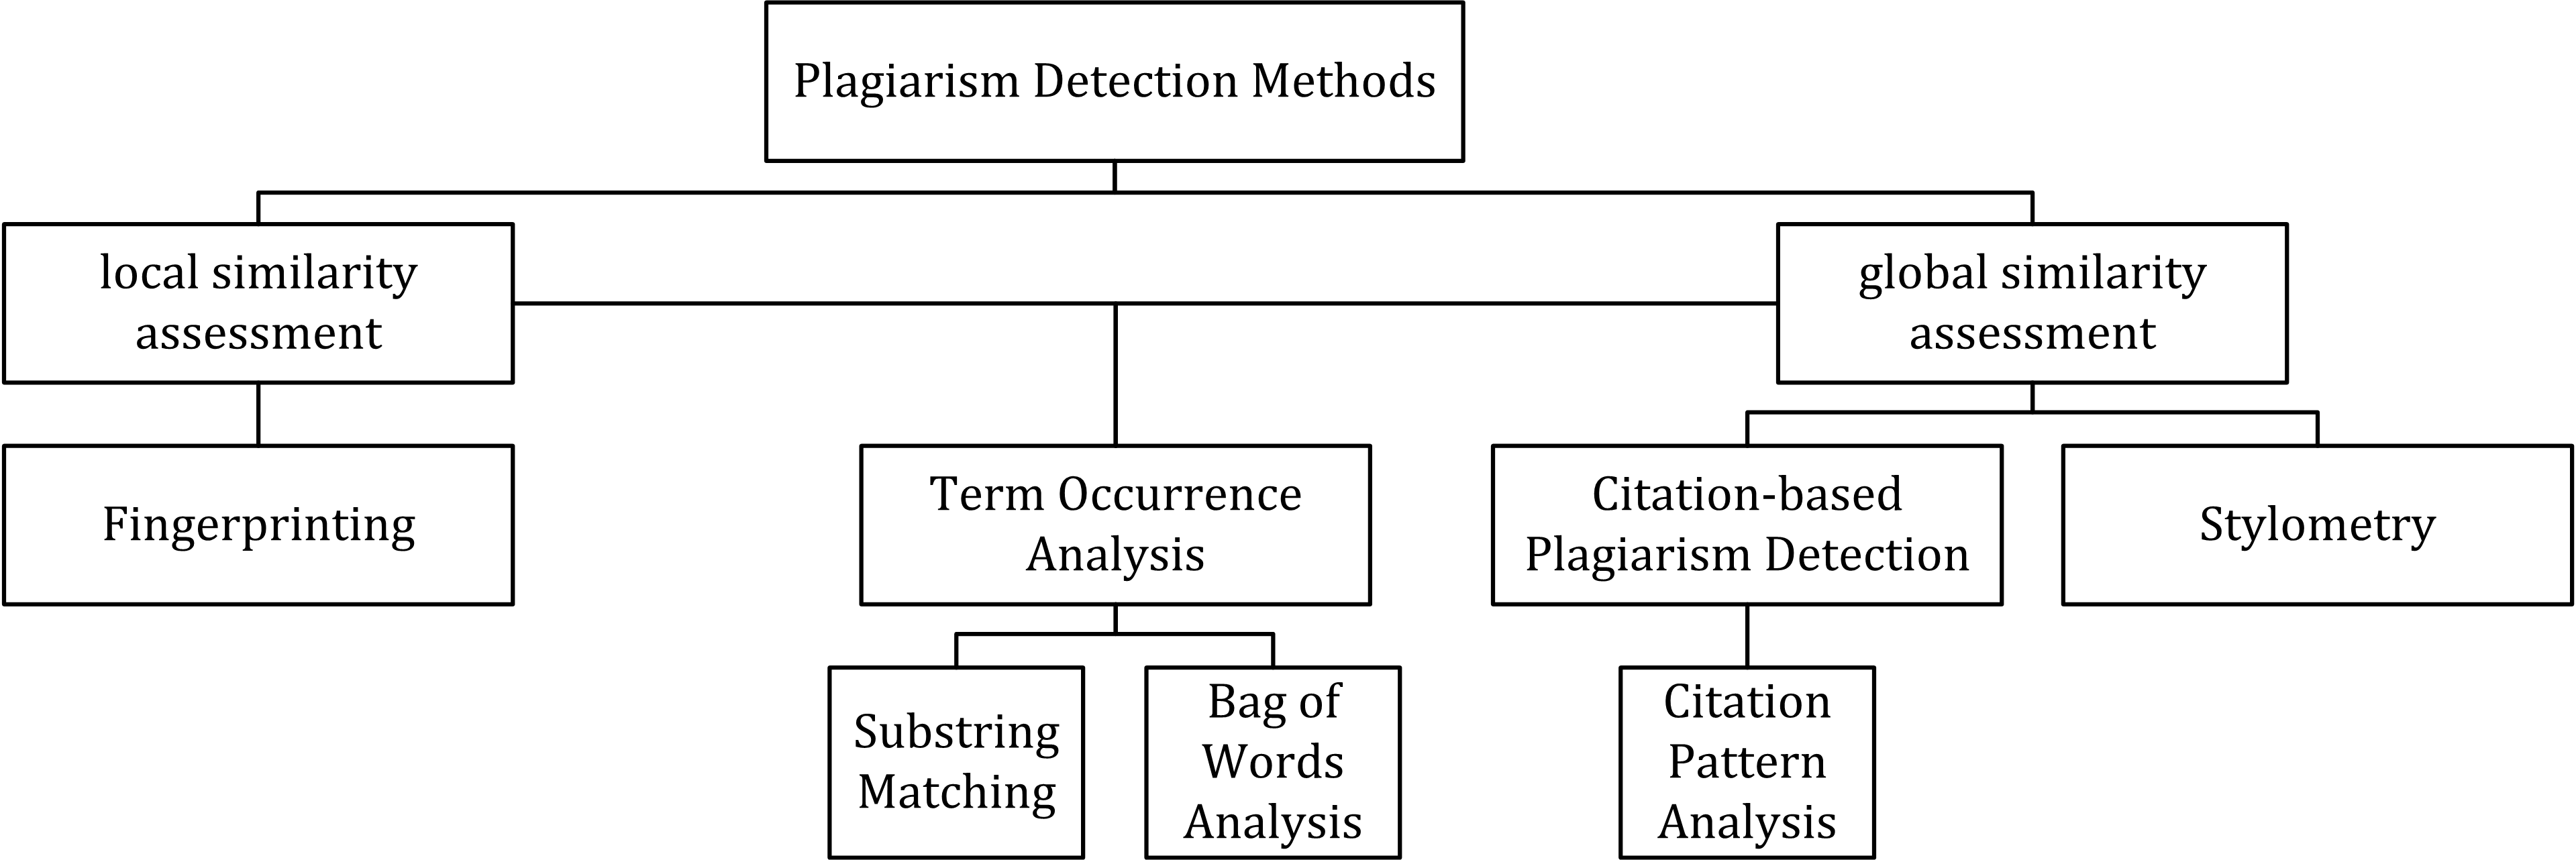
\includegraphics{figure/PDS_Classification}
\caption{Classification of computer assisted plagiarism detection methods as of Wikipedia. \cite{PDS_Classification}}
\end{figure}

%
%
%
\bibliographystyle{alpha}
\bibliography{refs}
\end{document}
